\documentclass[a4paper,11pt]{article}
\usepackage[utf8]{inputenc}
\usepackage{amsmath}
\usepackage{amssymb}
\usepackage[hidelinks]{hyperref}
\usepackage{geometry}
\geometry{margin=1in}
\usepackage{enumitem}
\usepackage{xcolor}
\usepackage{graphicx}
\usepackage{float}

\title{CSCib Lab Checklist}
\author{}
\date{}

\begin{document}
\maketitle

\section*{Cross-session checklist: preparing the working folder}

Applies to every laboratory session (L2, L3, and the following ones), before
starting any task in MATLAB.

\begin{enumerate}[label=$\square$, leftmargin=1.5em]
  \item Open MATLAB, confirming it is the correct version, \textbf{R2015a} (version
  8). If more than one version is installed on the laboratory PC, always choose
  this one, to guarantee compatibility with the rest of the work.

  \item Create, on the Desktop of the laboratory PC, a folder with an identifiable
  name, including the group number and the session. Example:
  \texttt{Desktop\textbackslash CSCib\_GroupXX\_L2}.

  \item Confirm that this folder has write permissions, by creating a test file
  inside it and deleting it afterwards. The guide explicitly asks that you use "a
  working folder with write permissions".

  \item Set that folder as the \emph{Current Folder} in MATLAB. Use the "Current
  Folder" field in the toolbar, or the command:
  \begin{verbatim}
cd('Desktop\CSCib_GroupXX_L2')
  \end{verbatim}
  Do not confuse this with "Set Path": that one tells MATLAB where to look for
  functions, not where to save files.

  \item Confirm the correct path before saving anything:
  \begin{verbatim}
pwd
  \end{verbatim}

  \item Always save data with the direct command. Example:
  \begin{verbatim}
save('input.mat', 'input')
  \end{verbatim}

  \item At the end of the session, copy the whole folder to the pen drive, and
  delete that folder from the laboratory PC (mandatory cleanup, requested by the
  guide).
\end{enumerate}

\section*{L2 checklist: sending commands to the motor (Section 3.3 of the guide)}

\textcolor{red}{\textbf{Safety warnings, valid from here on:}} keep a safe distance
from the flexible bar; always keep a finger near the power amplifier switch, to be
able to stop the motor; never let the bar rotate over itself.

\begin{enumerate}[label=$\square$, leftmargin=1.5em]
  \item Copy from the pen drive to the working folder (already created in the
  cross-session checklist) the \texttt{.slx} file built at home, with the model
  from steps 1 to 7 (Signal Generator connected to a Scope, with the signal saved
  to \texttt{input}). Open that file in MATLAB. There is no need to start the
  model from scratch, just keep building on it.

  \item Insert a D/A block: \texttt{Simulink Desktop Real-Time} $\to$
  \texttt{Analog Output}. Connect the Signal Generator to this block.

  \item Identify the installed data acquisition board: look at the back of the
  workbench computer and locate the board connector. If the connection is silver,
  the board is the \textbf{NI PCI-6221}. If the connection is blue, the board is
  the \textbf{NI MIO16E4}. Write down which one it is.

  \item Configure the D/A block: select the board identified in the previous step,
  sample time \texttt{0.001}, output channel \texttt{1}, voltage range from
  $-10$ to $10$ V, data type \texttt{volts}. \textcolor{red}{\textbf{The initial
  and final values must be exactly 0.}} If the final value is not zero, the motor
  keeps running without stopping after the experiment ends, and the equipment can
  be damaged.

  \item Configure the simulation to run in real time (\texttt{Ctrl+E}):
  \begin{itemize}
    \item Solver: Type = \texttt{Fixed-step}.
    \item Code Generation: System Target File = \texttt{rtwin.tlc}.
    \item Hardware Implementation: Device vendor = \texttt{Intel}, Device type =
    \texttt{X86/Pentium}.
  \end{itemize}

  \begin{figure}[H]
    \centering
    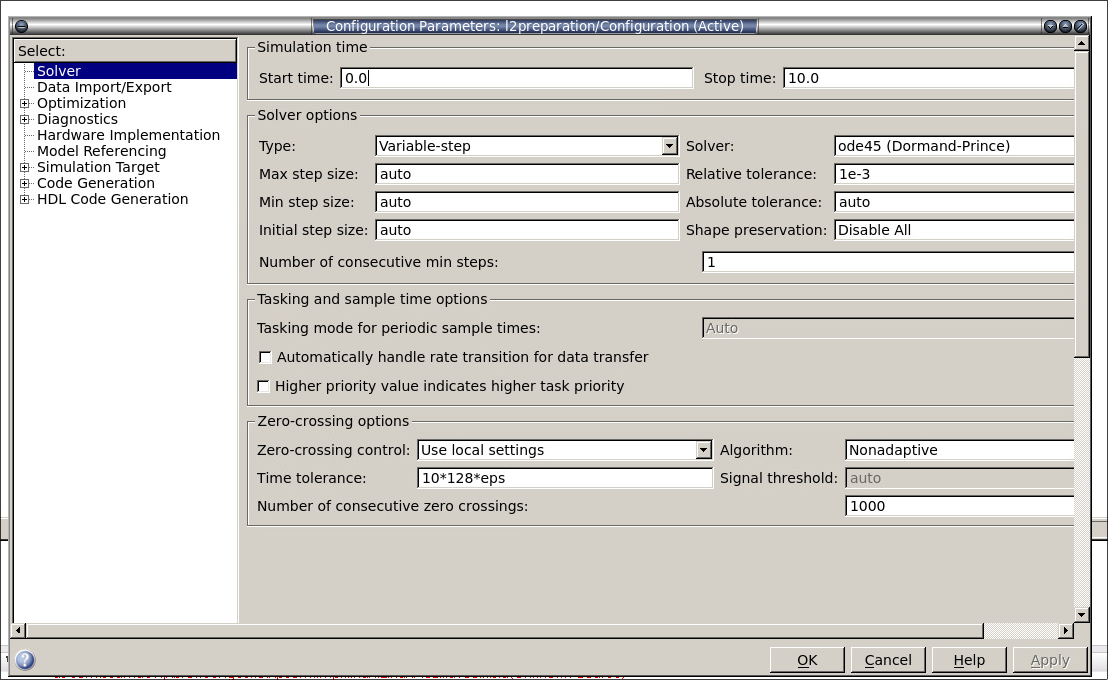
\includegraphics[width=0.85\textwidth]{Figs/l2_solver_config.png}
    \caption{\emph{Solver} panel inside \emph{Configuration Parameters}. In this
    screenshot \texttt{Type} is still set to \texttt{Variable-step} (the default
    value); change it to \texttt{Fixed-step}, as requested above.}
  \end{figure}

  \item Configure \emph{External} mode: menu \emph{Code}, then \emph{External
  Mode Control Panel}, then \emph{Signal \& Triggering}. Duration =
  \texttt{10001} samples (10 seconds at 1000 samples per second, plus the initial
  sample). Confirm, in the Simulink command bar, that the selected mode is
  \texttt{External}.

  \begin{figure}[H]
    \centering
    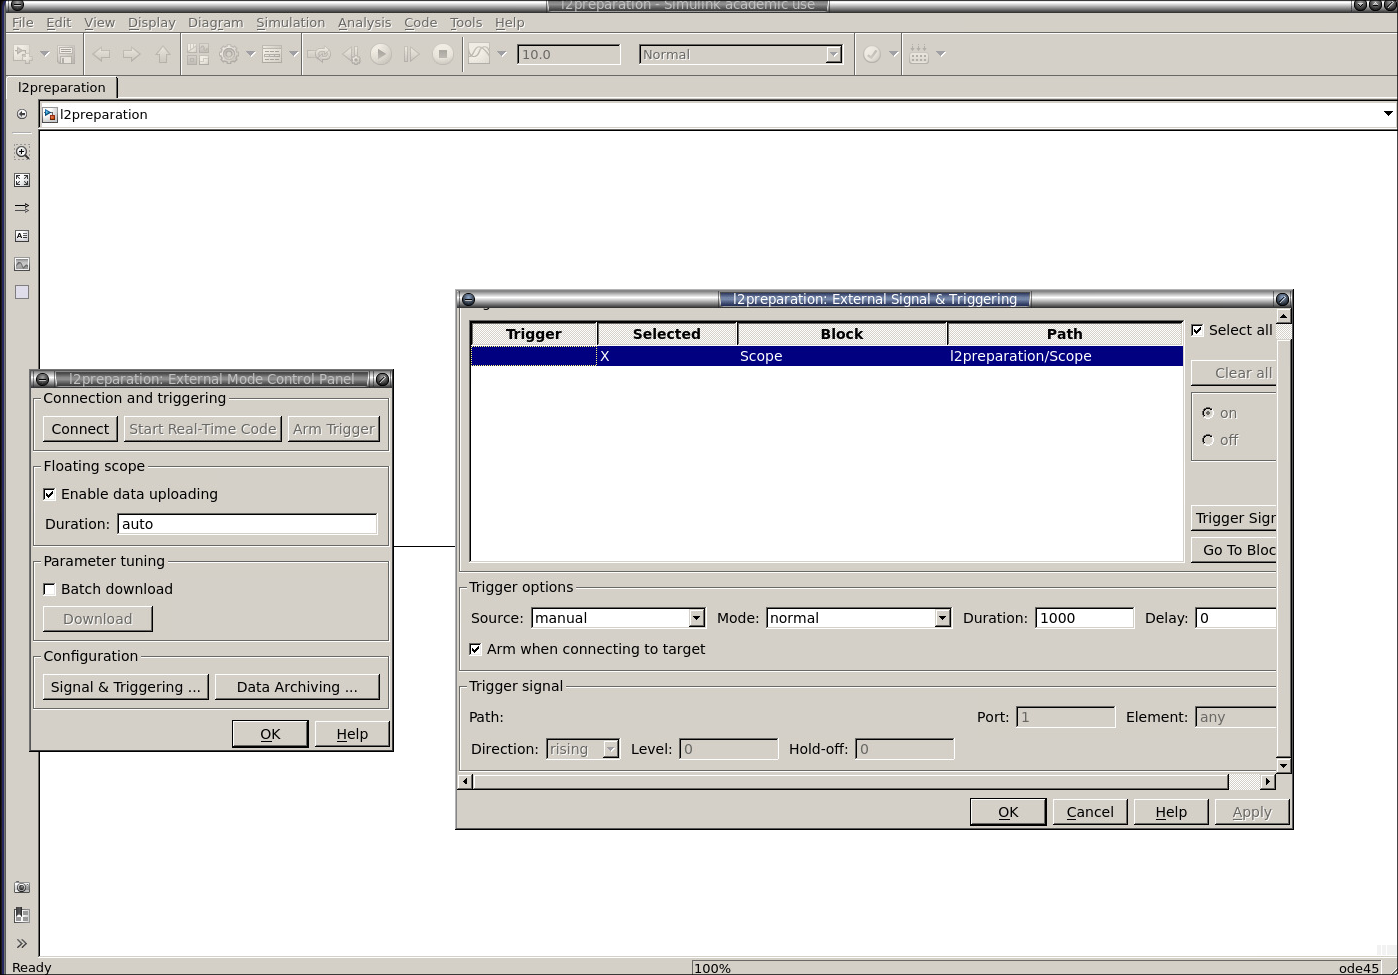
\includegraphics[width=0.95\textwidth]{Figs/l2_external_mode.png}
    \caption{\emph{External Mode Control Panel} (bottom left, accessed through the
    \emph{Code} menu) and \emph{External Signal \& Triggering} (right, button
    \emph{Signal \& Triggering...}). In this screenshot, \texttt{Duration} is set
    to \texttt{1000}; change it to \texttt{10001}, as requested above.}
  \end{figure}

  \item Save the project to the working folder.

  \item Ask the laboratory staff to confirm that everything is correctly
  configured, before running anything.

  \item Run the experiment (button $\blacktriangleright$). Observe the motor's
  behaviour: within each half period of the square wave, the applied voltage is
  constant, and over that interval the angular position does not stabilize, it
  keeps rising or falling continuously until the signal switches sign (the same
  effect already discussed in items (a) and (b) of Q1, and illustrated in Figure
  11 of the guide). Stop with the button $\blacksquare$ when needed. Record what
  was observed.

  \item At the end, follow the last two points of the cross-session checklist
  again: copy the working folder to the pen drive, and delete it from the
  laboratory PC.
\end{enumerate}

\section*{L3 checklist: reading sensors and calibration (Sections 3.4 and 3.5 of
the guide)}

Safety warnings: the same as in the L2 section, valid here too.

\begin{enumerate}[label=$\square$, leftmargin=1.5em]
  \item Copy from the pen drive to this session's working folder the \texttt{.slx}
  file from L2 (already with the Signal Generator and the D/A block configured).
  Open that file and keep building on it, without starting from scratch.

  \item Insert an A/D block for the potentiometer: \texttt{Simulink Desktop
  Real-Time} $\to$ \texttt{Analog Input}. Configure it: select the acquisition
  board identified in L2, sample time \texttt{0.001}, input channel \texttt{1}
  (potentiometer), voltage range from $-10$ to $10$ V, data type \texttt{volts}.

  \item Insert a Scope block to show the sensor signal, configured the same way as
  the L2 Scope (sample time \texttt{0.001}, "Save data to workspace" enabled).
  Name the variable \texttt{tensao\_pot}.

  \item Ask the laboratory staff to confirm before running. Run the experiment,
  observe the graph of the potentiometer voltage over time, and confirm that the
  variable \texttt{tensao\_pot} is available in the MATLAB workspace. Save:
  \begin{verbatim}
save('tensao_pot.mat', 'tensao_pot')
  \end{verbatim}

  \item \textbf{$K_p$ calibration (with the bar removed from the motor):} remove
  the bar from the motor shaft before continuing.

  \item Apply a $1$ V step to the motor (the same D/A block, now with a constant
  value instead of the Signal Generator) and let the motor spin freely for a few
  seconds, recording \texttt{tensao\_pot} continuously.

  \item In MATLAB, process the data to obtain $K_p$:
  \begin{enumerate}[label=(\alph*)]
    \item Detect the reset instants in the signal (where the voltage jumps from
    one extreme to the other), using \texttt{diff} and a suitable threshold.
    \item Discard the first cycle (the motor is still in its start-up transient).
    \item Fit a straight line to the points (reset instant, accumulated number of
    rotations $\times$ $360^\circ$) to estimate the angular velocity $\omega$,
    using all the detected resets.
    \item Compute, for each sample, the local reference angle
    $\theta_{\text{ref}}(t) = \omega \cdot (t - t_k)$, where $t_k$ is the reset
    immediately before the sample.
    \item Fit, by least squares, $\theta_{\text{ref}} = K_p \cdot \theta_e +
    \text{offset}$, pooling the data from all cycles together (\texttt{polyfit}
    or the \texttt{\textbackslash} operator).
  \end{enumerate}

  \item \textbf{$K_e$ calibration (bar on the calibration rig, not on the motor):}
  mount the bar on the rig with the calibration comb, and connect the cable to the
  strain gage (not to the potentiometer).

  \item Keep working on the same base model (do not create a new file): add an
  \texttt{Analog Input} block for the strain gage, joining the Signal Generator,
  the D/A block, and the potentiometer's Analog Input block already present,
  exactly as in Figure 10 of the guide. The Signal Generator and the D/A block
  serve no relevant purpose in this calibration (the bar is disconnected from the
  motor), but there is no need to remove them.

  \begin{figure}[H]
    \centering
    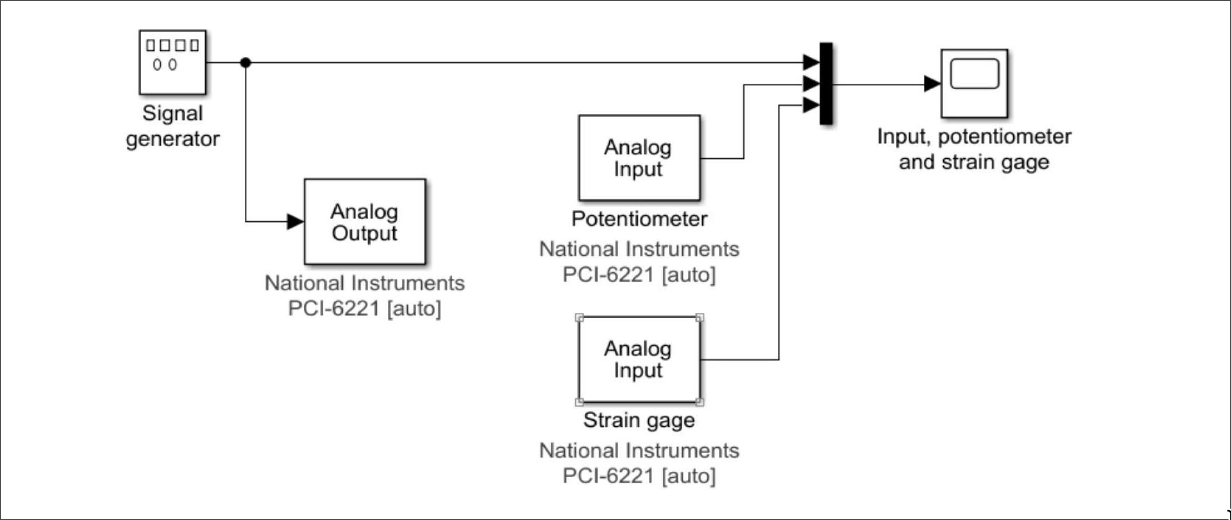
\includegraphics[width=0.95\textwidth]{Figs/l3_full_diagram.png}
    \caption{Full diagram (Figure 10 of the guide): Signal Generator connected to
    the D/A block (\emph{Analog Output}), and two \emph{Analog Input} blocks, one
    for the potentiometer and one for the strain gage, both joined in a Mux before
    the final Scope.}
  \end{figure}

  \item Configure the new A/D block, with the same parameters as the
  potentiometer's block (step 15 of the guide): sample time \texttt{0.001},
  voltage range from $-10$ to $10$ V, data type \texttt{volts}.
  \textbf{Warning:} the guide does not state the strain gage's channel number in
  writing (only the potentiometer's, channel \texttt{1}). Confirm the correct
  channel at the bench (connector label, or ask the laboratory staff) before
  choosing it in the block.

  \item Insert a Scope block (or a display) connected to this new A/D block, to
  read the strain gage voltage.

  \item For each slot of the comb, deflect the bar to that slot and record the
  corresponding electrical tension. Compute the deflection angle of each slot with
  $\alpha_{\text{[degree]}} = \frac{180}{\pi} \cdot \frac{D}{L}$, with $D$ the
  deflection distance of the slot and $L$ the length of the bar.

  The comb's slots are spaced at intervals of $1/4$ inch ($0.635$ cm $= 6.35$ mm),
  so the deflection distance of slot number $n$ (counted from the rest position)
  is:
  $$D_n = n \times 6.35 \text{ mm}$$

  Use the following table (filled in by hand, quickly, at the bench):

  \begin{table}[H]
    \centering
    \renewcommand{\arraystretch}{2.2}
    \begin{tabular}{|c|c|c|c|}
      \hline
      \textbf{Slot} & \textbf{$D$ (mm)} & \textbf{$\alpha$ (degree)} &
      \textbf{Measured tension (V)} \\
      \hline
       & & & \\
      \hline
       & & & \\
      \hline
       & & & \\
      \hline
       & & & \\
      \hline
       & & & \\
      \hline
       & & & \\
      \hline
       & & & \\
      \hline
       & & & \\
      \hline
       & & & \\
      \hline
       & & & \\
      \hline
    \end{tabular}
    \caption{$K_e$ calibration table: comb deflection against measured tension.}
  \end{table}

  \item With the $(\alpha, \text{tension})$ pairs from the table, fit by least
  squares $\alpha = K_e \cdot \alpha_e + \text{offset}$ in MATLAB, and save the
  raw data used in the fit.

  \item At the end, follow the last two points of the cross-session checklist
  again: copy the working folder to the pen drive, and delete it from the
  laboratory PC.
\end{enumerate}

\end{document}
